
\usepackage[utf8]{inputenc}
%\usepackage[top=0.5in, bottom=0.5in, left=1in, right=1in]{geometry}

\usepackage{natbib}
\usepackage{graphicx}

\usepackage{amssymb}
\usepackage{amsthm}
\usepackage{amsfonts}
\usepackage{amsmath} 
\usepackage[usenames,dvipsnames]{xcolor}
\usepackage{tikz}
\usepackage{pgf}
\usepackage{pgflibraryarrows}
\usepackage{pgffor}
\usepackage{pgflibrarysnakes}
\usepackage{todonotes}


\usetikzlibrary{fit} % fitting shapes to coordinates
\usetikzlibrary{backgrounds} % drawing the background after the foreground
\usetikzlibrary{patterns}
\usetikzlibrary{positioning}
\tikzstyle{background}=[rectangle,fill=gray!10, inner sep=0.1cm, rounded corners=0mm]
\usepgflibrary{shapes}
\usetikzlibrary{snakes,automata}
\usetikzlibrary{shadows}


%\tikzstyle{nloc}=[draw, text badly centered, rectangle, rounded corners, minimum size=2em,inner sep=0.5em]
\tikzstyle{background}=[rectangle,fill=gray!10, inner sep=0.1cm, rounded corners=0mm]
\tikzstyle{loc}=[draw,rectangle,minimum size=1.4em,inner sep=0em]
\tikzstyle{trans}=[-latex, rounded corners]
\tikzstyle{trans2}=[-latex, dashed, rounded corners]


\newcommand{\tool}{\texttt{Hybrolic}}

\newcommand{\set}[1]{\left\{ #1 \right\}}
\newcommand{\Set}[1]{\big\{ #1 \big\}}
\newcommand{\seq}[1]{\langle #1 \rangle}
\newcommand{\Nat}{\mathbb N}
\newcommand{\Q}{\mathbb Q}
\newcommand{\R}{\mathbb R}
\newcommand{\Real}{\R}
\newcommand{\Int}{\mathbb Z}
\newcommand{\Rat}{\mathbb Q}
\newcommand{\Rplus}{\R_{\geq 0}}
\newcommand{\Zpos}{\Int_{\geq 0}}


\newcommand{\Reach}{\textsc{Reach}}
\newcommand{\Sched}{\textsc{Sched}}
\newcommand{\LTLMC}{\textsc{LTL-MC}}
\newcommand{\PSPACEC}{\textsc{Pspace-Complete}}
\newcommand{\PSPACE}{\textsc{Pspace}}
\newcommand{\EXPTIMEC}{\textsc{Exptime-Complete}}
\newcommand{\EXPTIME}{\textsc{Exptime}}
\newcommand{\NPC}{\textsc{NP-Complete}}
\newcommand{\NLC}{\textsc{NL-Complete}}
\newcommand{\NLOGS}{\textsc{Nlogspace}}
\newcommand{\UNDEC}{\textsc{Undecidable}}
\newcommand{\EXPTIMEH}{\textsc{Exptime-Hard}}
\newcommand{\PTIME}{\textsc{Ptime}}
\newcommand{\PTIMEC}{\textsc{Ptime-Complete}}


\newcommand{\ptime}{{\sc P}\xspace}
\newcommand{\E}{{\bf E}}
\newcommand{\A}{{\bf A}}
%\DeclareMathOperator{\interior}{int}
\newcommand{\norm}[1]{\|#1\|}

\newcommand{\point}[1]{{\overline{#1}}}
\newcommand{\bbQ}{\mathbb{Q}}
%\DeclareMathOperator*{\opt}{opt}
\newcommand{\modenum}{|M|}
\newcommand{\ps}{\point{s}}
\newcommand{\pt}{\point{t}}
\newcommand{\px}{\point{x}}
\newcommand{\py}{\point{y}}
\newcommand{\pz}{\point{z}}
\newcommand{\vv}{\vec{v}}
\newcommand{\vw}{\vec{w}}
\newcommand{\vb}{\vec{b}}
\newcommand{\vf}{\vec{f}}
\newcommand{\vt}{\vec{t}}
\newcommand{\vr}{\vec{r}}
\newcommand{\vp}{\vec{p}}
\newcommand{\vn}{\vec{n}}
\newcommand{\pc}{\point{c}}

\newcommand{\vzero}{\vec{0}}
\newcommand{\Rmax}{{R_{\textrm{max}}}}
\newcommand{\Rmin}{{R_{\textrm{min}}}}
\newcommand{\dmax}{d_{\textrm{max}}}
\newcommand{\dint}{d}

\newcommand{\facet}[2]{#1|_{#2}}
\newcommand{\rows}[1]{\mathit{rows}(#1)}
\newcommand{\ball}[2]{B_{#1}(#2)}

\newcommand{\inv}{\mathit{Inv}}
\newcommand{\dia}{\mathit{dia}}
\newcommand{\act}{\mathit{Act}}
\newcommand{\enb}{\mathit{Enb}}
\newcommand{\reset}{\mathit{Rst}}
\newcommand{\sem}[1]{ [ \! [ {#1}  ]  \! ]} % semantic brackets

\newcommand{\Aa}{\mathcal{A}}
\newcommand{\Dd}{\mathcal{D}}
\newcommand{\lval}{\text{\it lval}}
\newcommand{\uval}{\text{\it uval}}
\newcommand{\Ee}{\mathcal{E}}
\newcommand{\Hh}{\mathcal{H}}
\newcommand{\Pp}{\mathcal{P}}
\newcommand{\Gg}{\mathcal{G}}
\newcommand{\Cc}{\mathcal{C}}
\newcommand{\Ff}{\mathcal{F}}
\newcommand{\N}{\mathbb{N}}
\newcommand{\Rr}{\mathcal{R}}
\newcommand{\Mm}{\mathcal{M}}
\newcommand{\Tt}{\mathcal{T}}
\newcommand{\Vv}{\mathcal{V}}
\newcommand{\hTt}{\hat{\mathcal{T}}}
\newcommand{\sTt}{\sem{\mathcal{T}}}
\newcommand{\sGamma}{\sem{\Gamma}}
\newcommand{\hS}{\hat{S}}
\newcommand{\hA}{\hat{A}}
\newcommand{\hT}{\hat{T}}

\newcommand{\rect}{\textrm{rect}}
\newcommand{\poly}{\textrm{poly}}
\newcommand{\sing}{\textrm{sing}}
\newcommand{\oct}{\textrm{oct}}
\newcommand{\pred}{\textrm{pred}}

\newcommand{\PROB}{\text{\it Prob}}
\newcommand{\eE}{\mathbb{E}}
\newcommand{\bB}{\mathbb{B}}
\newcommand{\iI}{\mathbb{I}}
\newcommand{\tT}{\mathbb{T}}

\newcommand{\Trace}{\mathsf{\it Trace}}

\newcommand{\until}{\:\mathcal{U}}

\theoremstyle{theorem}
\newtheorem{theorem}{Theorem}[section]

\theoremstyle{definition}
\newtheorem{definition}{Definition}[section]

\theoremstyle{definition}
\newtheorem{example}{Example}[section]

\title{Concolic Testing for Analysis of Hybrid Systems  \\
\large CS477 Project Report}
\author{Umang Mathur \and Atul Sandur}
\date{November 9, 2015}

\begin{document}

\maketitle

\section{Introduction}
Hybrid automata provide a generic framework for modeling embedded systems with continuous and dense variables, such as controllers for plants, reactors or for robot motion planning.
It is often meaningful to ask questions such as whether a given hybrid system reaches some \emph{error} state. For safety critical systems such as nuclear power plants, it becomes quite important to verify that the system does not crash. There is a rich literature on verification of hybrid systems to tackle this problem. However, it turns out that the general model of Hybrid automata is quite expressive and not surprisingly, very simple questions like reachability are undecidable, and heuristics based techniques for answering such verification questions are not known to scale well.
As part of this project, we intend to develop systematic techniques for answering questions such as reachability of some state in hybrid systems, using concepts from automated test input generation.

\section{Hybrid Automata}
The framework of Hybrid automata, introduced by Alur, Courcourbetis, Henzinger, and Ho~\cite{ACH92}, provides a formal modeling and analysis environment to analyze the interaction between the discrete and the continuous parts of cyber-physical systems. Hybrid automata can be considered as generalization of finite state automata augmented with a finite set of real-valued variables whose dynamics in each state is governed by a system of ordinary differential equations. Moreover, the discrete transitions of hybrid automata are guarded by constraints over the values of these real-valued variables, and enable discontinuous jumps in the evolution of these variables. 
In its full generality, the reachability question for Hybrid automata is undecidable. In fact the question remains undecidable for very simple subclasses of Hybrid automata, when the rate of evolution of variables are restricted to be constant integer values, and the constraints in the system are simple linear constraints.



%\begin{figure}[h!]
%\centering
%\includegraphics[scale=1.7]{universe.jpg}
%\caption{The Universe}
%\label{fig:univerise}
%\end{figure}

\section{Concolic Testing}
Concolic testing~\cite{SEN07} automates test input generation by combining concrete and symbolic executions of the system under test. So the concrete part constitutes normal execution of the program while symbolic part collects symbolic constraints over the symbolic input values at each branch point encountered along concrete execution path. At the end of an execution, we have collected a set of path constraints that exercise an execution path in the system. For the next iteration, one of the constraints is negated and solved using constraint solvers to generate a new test input that directs the system along a different execution path. This process continues until all feasible distinct execution paths have been explored. When some of the symbolic constraints become too complicated for the constraint solver to generate concrete values, they are simplified by replacing some of the symbolic values with concrete values.
Concolic testing is thus sound (infers real bugs) and also allows exploring previously unreachable paths in the system. 

\section{Approach}
To begin with, we will model embedded systems using Singular Hybrid Automata (SHA), the reachability question for which is known to be undecidable even for 3 vartiables~\cite{HKPV98}. SHA can be described as a set of discrete states and a set of continuous variables. Additionally there is a function $f(s,x)$ which is a constant integer for every discrete state $s$ and continuous variable $x$, that denotes the rate of evolution of $x$ in state $s$. Moreover every state $s$ and discrete transition between any two such states are annotated using a set of linear constraints. The constraints are referred to as \emph{invariants} and \emph{guards} respectively. A sequence of pairs of the form ($s$,$t$) where $s$ is a discrete state and $t$ is positive constant denoting time spent in that state, describes a valid \emph{trace} if all guards and invariants are met throughout the sequence. We say that a state $q$ is reachable, if there is some initial value for the continuous variables and a finite trace $(s_0, t_0), (s_1, t_1),\ldots (s_k,t_k)$ exists such that $s_k = q$. 

\begin{figure}[h]
  \begin{center}
    \scalebox{0.7}{
    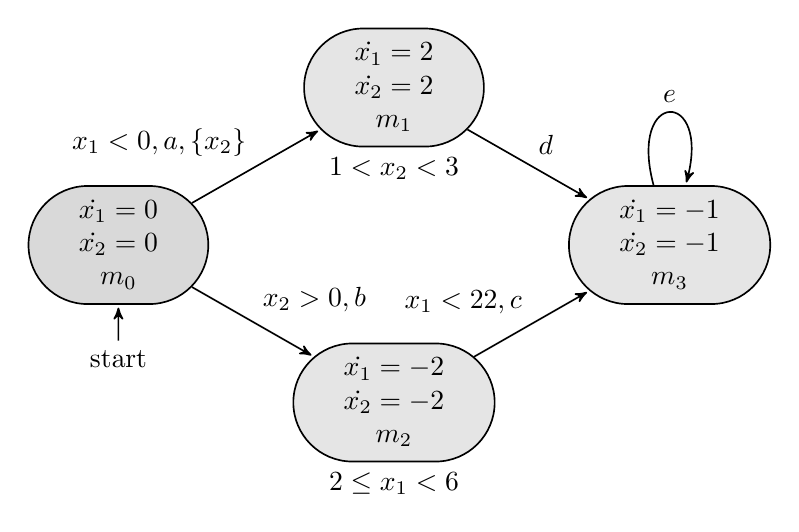
\begin{tikzpicture}[->,>=stealth',shorten >=1pt,auto,semithick]
      \tikzstyle{every state}=[fill=gray!20!white,minimum size=3em,rounded rectangle]
      
      \node[initial, initial where=below,state,fill=gray!30] at (0, 0) (m0) {$\begin{array}{c}
          \dot{x_1} = 0 \\ \dot{x_2} = 0 \\ m_0 \end{array}$};
      
      \node[state, label=below:$1< x_2 < 3$] at (3.5, 2) (m1) {$\begin{array}{c}
          \dot{x_1} = 2\\ \dot{x_2} = 2  \\ m_1 \end{array}$} ;
      
      \node[state, label=below:$2 \leq x_1 < 6$] at (3.5, -2) (m2) {$\begin{array}{c} \dot{x_1} = -2 \\ \dot{x_2} = -2 \\ m_2 \end{array}$} ;
      
      \node[state] at (7, 0) (m3) {$\begin{array}{c} \dot{x_1} = -1 \\ \dot{x_2} = -1  \\ m_3 \end{array}$} ;
  
      \path (m0) edge node {$x_1 < 0, a, \set{x_2}$} (m1);
      \path (m0) edge node[] {$x_2 > 0, b$} (m2);
      
      \path (m2) edge node[] {$ x_1 < 22, c$} (m3);
      \path (m1) edge node[] {$d$} (m3);
   
      \path (m3) edge [loop above] node[] {$e$} (m3);
    \end{tikzpicture}
  }
\end{center}
\label{fig:sha}
  \caption{Singular Hybrid Automata with four modes and two variables.} 
\end{figure}

Given initial values of continuous variables and a concrete trace, it is easy to check if it is a valid trace that reaches some state $q$. However coming up with concrete values for time durations in that trace is non-trivial because the possible values of $t_i$'s are uncountable. Therefore it makes sense to look at symbolic traces where $t_i$'s are symbolic variables. 

A very basic idea to solve reachability question using test generation concepts, is to collect constraints on invariants/guards in a given symbolic trace and feed it to a suitable solver to check for feasibility of the constraints. This will give concrete initial values for the input to the system. It is possible to avoid quantifiers from the constraints because the continuous variables evolve in a linear fashion relative to each other. Therefore we expect simple SMT solvers like Yices to be able to handle these constraints. The challenge is in determining correct symbolic traces that lead to a final goal state in hybrid sytems which have loops. This is because one can generate infinite number of symbolic traces as inputs to our algorithm. We will initially focus our attention on bounded step reachability. Another challenging aspect is to be able to deal with non-linear invariants/guards as constraints that most solvers cannot handle. We attempt to attack this problem by guiding symbolic executions using concrete values for symbolic variables. This is primarily where we will use concepts from concolic testing techniques. Further, such non-linear constraints result in quantified constraints which have one or more quanitified variables. This is again difficult for constraint solvers to handle.  
For hybrid systems where continuous variables evolve in a much complex fashion, such as when the rates of evolution are specified in terms of arbitrary differential equations, there are many more challenges that need to be addressed. We will be looking at such problems as part of future work.  

\bibliographystyle{plain}
\bibliography{references}
\end{document}
